\chapter{Bases technologiques}
Ce chapitre permet de présenter quelques bases théoriques nécessaires à la bonne compréhension de ce travail. 

\section{Traitement d'images}
\subsection{Représentation d'une image}\label{techno.traitement.repr}
Une image est formée de pixel. La figure \ref{fig:pixels} présente une image d'une taille de 104x71 pixels, où ceux-ci peuvent donc être distingués les uns des autres.

\begin{figure}[ht]
    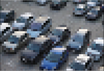
\includegraphics[width=50mm]{img/bases_technologiques/pixels.png}
    \centering
    \caption{Image de faible définition dont les pixels sont apparents}
    \label{fig:pixels}
\end{figure}

Chaque pixel d'une image couleur est généralement constitué de 3 valeurs\footnote{Parfois, une composante de transparence peut aussi être présente. Dans certains cas bien spécifiques, il peut même être possible d'y inclure des composantes telles que la profondeur (la distance entre la caméra et l'objet désigné par le pixel), ou encore la température (caméra thermique).}: une composante rouge, une verte et une bleue, qui permet de décrire la couleur associé à ce pixel. En traitement d'image, ces composantes RGB\footnote{\textit{RGB}: \textit{Red Green Blue} pour \textit{rouge vert bleu}} sont souvent décrites comme des canaux\footnote{\textit{channel}, mot anglais, est aussi utilisé.} différents.

\begin{figure}[ht]
    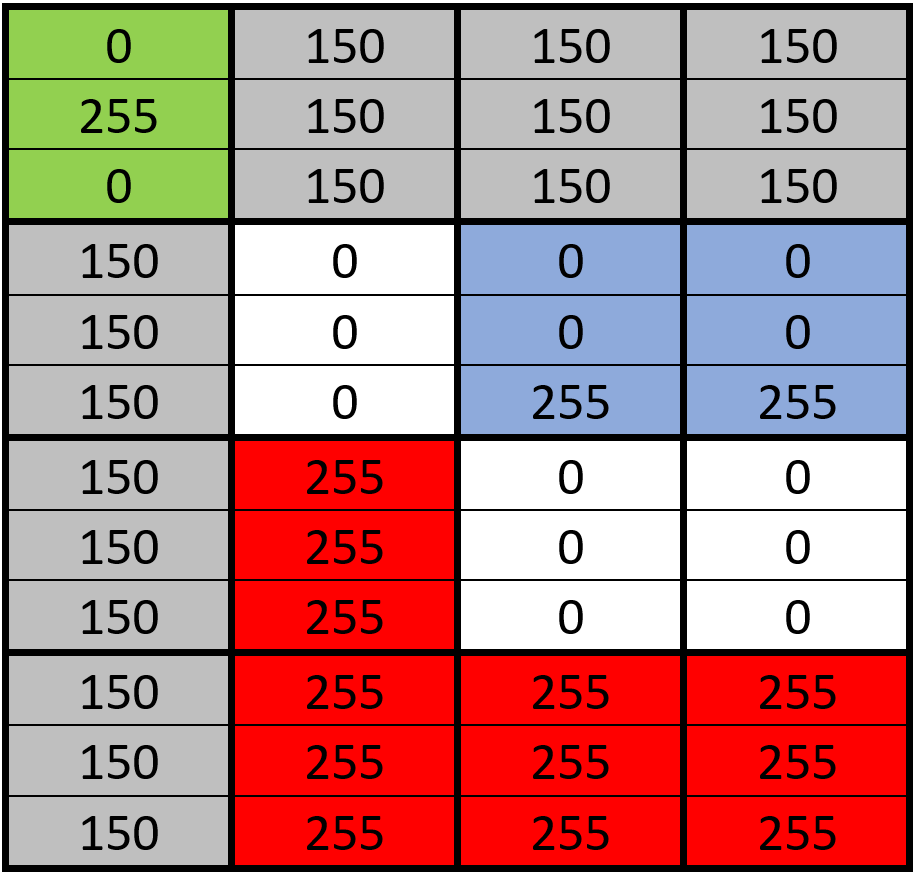
\includegraphics[width=50mm]{img/bases_technologiques/images_pixels.png}
    \centering
    \caption{Représentation d'une image couleur 4x4 pixels et les composantes rouges, vertes, et bleues}
\end{figure}

Une image couleur peut donc être représentée en mémoire à l'aide d'un tableau à 3 dimensions. 2 normes différentes peuvent être utilisées:
\begin{description}
    \item[Canal en premier (\textit{channel first})] Le canal est désigné par la première dimension. Ainsi, pour une image couleur de 4x4 pixels, le tableau est de la forme 3x4x4.
    \item[Canal en dernier (\textit{channel last})] Le canal est désigné par la dernière dimension. Pour une image couleur de 4x4 pixel, le tableau est de la forme 4x4x3.
\end{description}

Dans ce projet, il a été défini que le format \textit{canal en dernier} sera utilisé en priorité. 

\subsubsection{Espace de couleur}\label{techno.traitement.repr.coul}
En section précédente, le format RGB a été présenté. Il est cependant important de noter qu'il existe d'autres modèles permettant de représenter une couleur. Notamment, le modèle HSV (\textit{Hue, Saturation, Value}, en français \textit{TSV} pour \textit{teinte, saturation, valeur}) a été utilisé dans ce travail. \autocite{wiki:HSV} 

\begin{figure}[ht]
    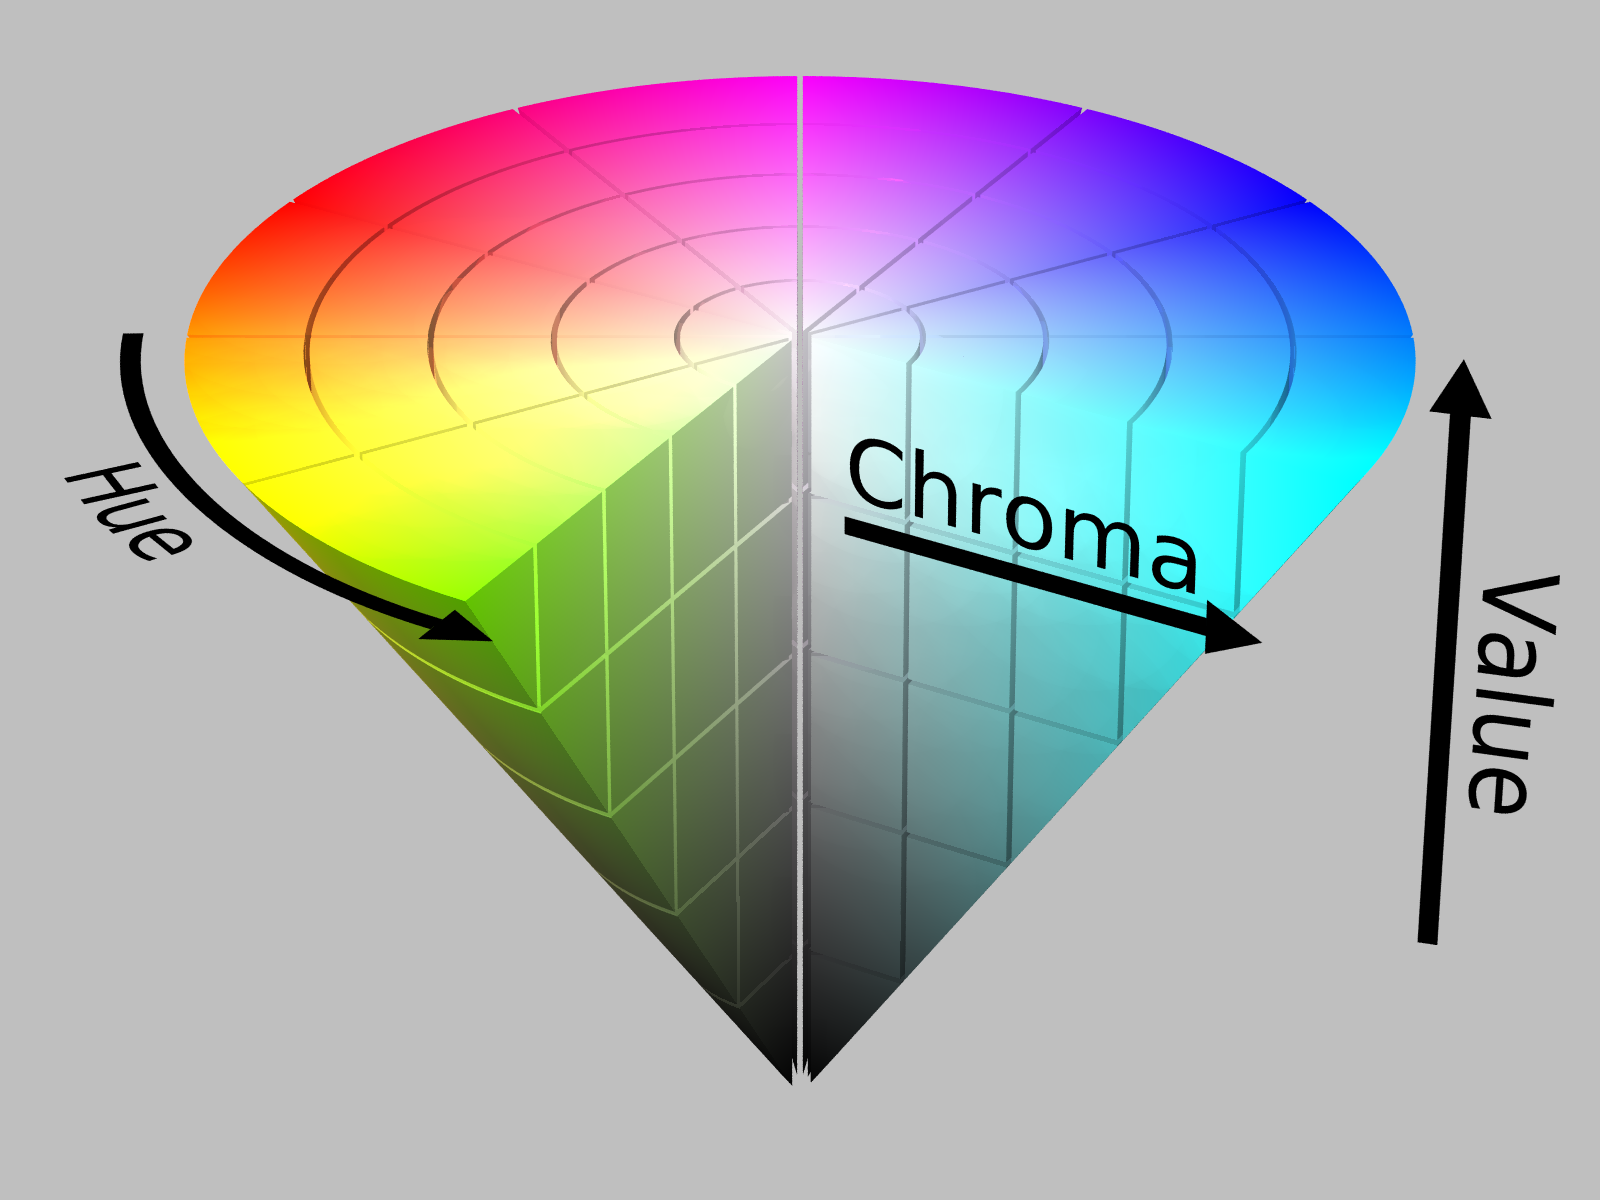
\includegraphics[width=70mm]{img/bases_technologiques/HSV.png}
    \centering
    \captionsource{Cône représentant l'espace HSV. Ici, la saturation est désignée par le terme \textit{Chroma}}{wiki:HSV}
\end{figure}

La teinte d'une couleur pouvant être obtenue grâce à l'aide d'un canal unique, cette représentation peut sembler idéale dans certains cas, permettant de mieux distinguer les couleurs entre elles. Notamment, cet espace de couleur a été utilisé lors des tests de détection de bords tel que décrit en section \ref{conception.traitement} \itnameref{conception.traitement}.

\subsection{Sous-échantillonnage}
Une image d'un certain nombre de pixel en largeur et en hauteur peut être redimensionnée. En traitement d'images\footnote{Le sur- et sous-échantillonnage sont en réalité utilisés pour toutes données décrites à l'aide d'échantillons ou une discrétisation, comme par exemple les fichiers audios.}, on parle de:
\begin{description}
    \item[Sur-échantillonnage (\textit{Oversampling})] La résolution de l'image est augmentée, le nombre de pixels qui y sont présents est donc supérieur. 
    \item[Sous-échantillonnage (\textit{Downsampling})] La résolution de l'image est réduite, le nombre de pixels qui y sont présents est donc diminué. 
\end{description}

Il faudra noter que la réduction de la résolution d'une image induit irrémédiablement à une perte d'information. 


\subsection{Détection de bord}
\todo{Parler du fait qu'on peut séparer chacun des canaux de limage pour faire de la convolution, mais qu'on peut 1 séparer, 2 faire la conv séparément, 3 les remettres ensembles}

\section{Réseau de neurones à convolutions}
\subsection{\textit{Machine Learning}}
\todo{Parler des 3 types de machines learning (supervisé, non supervisé, semi-supervisé)}

\subsection{Réseau de neurones}

\subsection{Convolution}\label{techno.traitement.convolution}


\todo{Détection d'objet}